%\documentclass[twocolumn]{amsart}
\documentclass[journal]{IEEEtran}
\usepackage{tikz, amsmath, amssymb,listings}
\begin{document}

\title{MAC address table flooding probability}

\author{Morten~Jagd~Christensen,~\IEEEmembership{Senior Member,~IEEE}% <-this % stops a space
\thanks{M. Christensen is with Cobham, e-mail: (see http://www.jcaps.com).}% <-this % stops a space
}


\markboth{Journal of \LaTeX\ Class Files,~Vol.~6, No.~1, January~2007}%
{Shell \MakeLowercase{\textit{et al.}}: Bare Demo of IEEEtran.cls for Journals}

\maketitle

\begin{abstract}
A simple but realistic model of the hashing mechanisms in an ethernet switch is presented. The probability 
of flooding is given as a function of various parameters. A discussion about size constraints and hashing functions
is done.
\end{abstract}

\section{Introduction}
\IEEEPARstart{A}{n} Ethernet network consists of several interconnected bridges
in a loop-free topology (using the Spanning Tree algorithm). In 
addition to other switches nodes (or end hosts) are also connected.
Each node is uniquely identified by its MAC address, which is a 48 bit 
serial number. The bridges ensures the delivery of packets to end-hosts
in a given segment. For unicast traffic the end-host is normally the only recepient 
of that packet. The forwarding mechanism is based on MAC address
tables holding enough information to make a forwarding descision,
where the switch ... at most one port... [1][2]

For this purpose, each bridge maintains a forwarding table with entries
of the form $<$MAC address, DPORT$>$. 
Populating the forwarding table is carried out based on the
{\em source addresses} of packets that a bridge receives. 

When subsequently receiving a packet on port P1 with an unknown
source address SA, the bridge then creates (learns) an entry of the form
$<$SA,P1$>$.

The 'learned' entries are then used to make forwarding
decisions for packets {\em destined} for address SA. These
will be sent out on port P1. Now if a packet arrives on 
any port, with a destination address DA which is not in the 
forwarding table, that packet is forwarded on all active ports.
This is also called flooding. Excessive flooding is a potentially big 
problem for the stability and bandwidth utilization in a network.

In the following we will describe a typical implementation of 
forwarding tables and the ...

While this analysis share some similarities with other studies,
these mostly seem to model traffic scenarios, where we look
at ...

\section{bins and buckets}
\IEEEPARstart{A}{} 
typical implementation of a MAC address forwarding table is 
to make an array of $W$ buckets or bins each able to hold a number
of MAC address entries. We call this number the depth $d$ of the table.

Thus the MAC address table has the size $d\cdot W \cdot c$ where $d$ is the size of the bin, $c$ is the size of a MAC addres plus additional 
information, and  $W$ is the number of bins. 


\begin{center}
\begin{tabular}{ll}
\hline
MAC & Port \\ 
\hline
00:23:14:00:00:01 &  3 \\
07:00:01:01:02:03 &  17 \\
\hline
\end{tabular}
\end{center}

Mapping a MAC address to a specific bin is typically done by applying a hashing 
function to the MAC address into the required number of buckets.

One popular method is to divide the MAC address into 4,6,8 or 12 bit chunks and then 
XOR these together. The final value identifies the bucket in which
the MAC address should be stored. Later we will discuss some specific hashing functions.




\section{Mac address hash collisions}

\IEEEPARstart{L}{et} us assume that the MAC address table in an Ethernet switch has the parameters $(W,d)$, where $W$ is the width of the 
address table and $d$ is the depth. Any incoming MAC address is hashed into one of $W$ slots and stored
in one of the $d$ entries. If two different MAC addresses hashes into the same slot we call it a (hash) collision.
 If the slot is already full the switch must replace an older entry with the new one or discard 
the new one. In either case this increases the likelihood that  



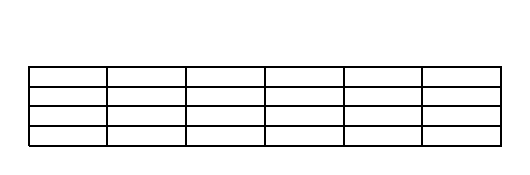
\begin{tikzpicture}[line width=0.75pt] 
\draw (0,0) -- (6,0) -- (6,1) -- (0,1) -- (0,0); 
\foreach \x in {1,...,5} \draw (\x,0) -- (\x,1);
\foreach \y in {0.25,0.5,...,0.75} \draw (0,\y) -- (6,\y);
\useasboundingbox (0,1.5);
\end{tikzpicture}

$MAC_{64} ->hash->M_{10}$

First we assume that MAC addresses are hashed into a uniform distribution. This means that any hash
value is equally probable. The actual distribution of MAC addresses is insignificant as long as the 
hashing function is sufficiently 'random' and that ... entropy ....
The probability for a MAC address to hash to slot $i$ is thus $p=1/M$. Now we will send $N$ different MAC addresses through
the switch, and
consider the probability for an arbitrary slot $i$ to contain zero, one or more entries after the experiment.

The experiment of hashing a single MAC address and observing wheter it is $i$ or not is called a Bernoulli experiment. 
Each individual Bernoulli experiment is a stochastic
variable $X$ which can have the value 0 if we hash to the value $i$, and 0 if not. 



We now repeate this Bernoulli experiment $N$ times and sums the outcomes to a new stochastic variable $Y$. 

$$
  Y = X_1 + X_2 + \cdots X_N
$$

It is easily shown that $Y$ is distributed according to the Binomial distribution $\mathbf{B}(N,p)$. 




$$
  P\{Y=n\} = \mathbf{B}(N,p) = \binom{N}{n}p^n(1-p)^{N-n}
$$
so the probability that the slot $i$ is empty (Y=0) after $N$ experiments is 
$$
   P\{Y=0\} = \binom{N}{0}p^0(1-p)^N = (1-p)^N
$$
if we as an example set $N=8000$ and $W=4096$ we get $(1-1/4096)^{8000} = 14.2\% $.

But how probable is it that all $d$ entries are occupied?
$$
  P\{Y>d\} = 1-P\{Y\le d\} = 1 - \sum_{k=0}^d P\{Y=k\}
$$

$$
  P_{flooding} = 1- \sum_{k=0}^d \binom{N}{k} p^k (1-p)^{N-k}
$$


\section{On HASH functions}
\IEEEPARstart{I}{n} the previous section we have assumed that 1) the distribution of 
MAC addresses is uniform or 2) that the output of the hashing algorithm
is sufficiently unpredictable. A fundamental paradigm of cryptography is that we can convert any distribution 
into a uniform distribution by means of a sufficiently effective hashing algorithm.

The various cryptographic hashfunctions MD4, MD5, SHA-1, SHA-256, etc. will certainly do the trick,
but these are often too computationally intensive or introduces latency which prevents wire-speed
forwarding.

\subsection{XOR}
The simplest hashing possible is the XOR method mentioned above. Although is is 
far from unpredictable it ...... 

$$h = MAC_1 \oplus MAC_2 \oplus MAC_3 \oplus MAC_4 \oplus MAC_5 \oplus MAC_6$$


\subsection{Pearson hashing}
Pearson hashing is a CBC-MAC using a lookup table, and produces an 8 bit hash
value.
\lstset{language=C, numbers=left,numberstyle=\tiny}
\begin{lstlisting}
h := 0
for each c in C loop
  index := h xor c
  h := T[index]
end loop
return h
\end{lstlisting}


\section{Simulations}
blah

\section{Conclusion}
When considering ,...

\section*{Acknowledgment}


The authors would like to thank...

\begin{thebibliography}{1}

\bibitem{IEEEhowto:kopka}
{\em Media Access Control Bridges}, IEEE Std 802.1D,2004.

\bibitem{IEEEhowto:kopka}
S.~Ray, R.~A.~Gue\'rin and R. Sofia, \emph{ADistributed Hash Table based Address
Resolution Scheme for Large-scale Ethernet Networks}, 3rd~ed.\hskip 1em plus
  0.5em minus 0.4em\relax University of Pennsylvania, 2007.

\end{thebibliography}

\end{document}
